\documentclass{article}

% if you need to pass options to natbib, use, e.g.:
%     \PassOptionsToPackage{numbers, compress}{natbib}
% before loading neurips_2020

% ready for submission
 %\usepackage{neurips_2020}

% to compile a preprint version, e.g., for submission to arXiv, add add the
% [preprint] option:
\usepackage[preprint]{neurips_2020}

% to compile a camera-ready version, add the [final] option, e.g.:
%\usepackage[final]{neurips_2020}

% to avoid loading the natbib package, add option nonatbib:
%\usepackage[nonatbib]{neurips_2020}

\usepackage[utf8]{inputenc} % allow utf-8 input
\usepackage[T1]{fontenc}    % use 8-bit T1 fonts
\usepackage{hyperref}       % hyperlinks
\usepackage{url}            % simple URL typesetting
\usepackage{booktabs}       % professional-quality tables
\usepackage{amsfonts}       % blackboard math symbols
\usepackage{nicefrac}       % compact symbols for 1/2, etc.
\usepackage{microtype}      % microtypography

% Added packages
\usepackage{amsmath,amssymb}
\DeclareMathOperator{\EX}{\mathbb{E}}% expected value
\usepackage{comment} % to comment out some codes
\usepackage{graphicx} % to insert some figures
\graphicspath{{figs/}} % to insert some figures
\usepackage{amsmath}


\title{Adaptive Quantitative Trading: An Imitative Deep Reinforcement Learning Approach}

% The \author macro works with any number of authors. There are two commands
% used to separate the names and addresses of multiple authors: \And and \AND.
%
% Using \And between authors leaves it to LaTeX to determine where to break the
% lines. Using \AND forces a line break at that point. So, if LaTeX puts 3 of 4
% authors names on the first line, and the last on the second line, try using
% \AND instead of \And before the third author name.

\author{%
  Chia-Hung Liao$^1$, Chia-Wei Hsu$^2$, Zhen-Yuan Hsu$^3$, Yu-Lin Lu$^4$\\
  
  \texttt{\{$^1$aiallen.cs07g, $^3$anson.cs08g\}@nctu.edu.tw}\\
  \texttt{\{$^2$music87.c, $^4$nycu309551038.cs09\}@nycu.edu.tw}\\
  Department of Computer Science\\
  National Chiao Tung University\\
}

\begin{document}
\maketitle


\section{Problem Overview}
\label{section:intro} %\ref{section:intro}

Please provide a brief overview of the selected paper. You may want to discuss the following aspects:
\begin{itemize}
    \item The main research problem tackled by the paper
    
    \item High-level description of the proposed method
\end{itemize}

There are three challenges in this paper. 
\begin{itemize}
\item Challenge 1: Noisy High-frequent Financial Data

First, the noisy high-frequent financial data. The market state is hard to be observed since the high-frequent financial data contain much noise. No one can know exactly whether the market is bullish or bearish, and whether it's time to buy or sell the security.

\item Challenge 2: Poor Generalization of Technical Analysis

Second, poor generalization of commonly used technical analysis. Even if the pattern of market reappears, the identical technical analysis may not be able to earn from the similar pattern again. Thousands of factor's interactions cause the market information indistinguishable.
%Considerable factors are affecting the market, and the interaction of them leads to indistinguishable information. 
To figure out this noisy information and improve generalization ability, machine learning gives the big-scale problem a chance to be solved. This paper seems the market as partially observable Markov decision process (POMDP) \citep{KAELBLING199899} and solves the process by recurrent deterministic policy gradient (RDPG) \citep{DBLP:journals/corr/HeessHLS15}, an off-policy deep reinforcement learning algorithm while deep learning concentrates on predicting the price trend and reinforcement learning focuses on constructing the best trading strategy.

\item Challenge 3: Balancing Exploration and Exploitation

But the reinforcement learning itself gives the third challenge, balancing exploration and exploitation. Because of the market friction like transaction fee, slippage, and market capacity, randomly explore the market without goals may cause great losses. However, a beneficial trading strategy is hard to get without enough trials and errors. To alleviate the trade-off problem, this paper uses imitative learning techniques, that is,  demonstration buffer and behavior cloning while the former learns from the technical index, Dual Thrust and the latter sets a prophetic trading expert which will take a daily sub-optimal action to execute. Overall, the whole three challenges can be tackled by the proposed method from this paper, imitative Recurrent Deterministic Policy Gradient (iRDPG) which contains imitative technique and RDPG algorithm. 
\end{itemize}

\section{Background and The Algorithm}
\label{section:algorithm}
Please present the essential background knowledge and the algorithm in this section. You may also describe the notations and the optimization problem of interest.

\subsection{Problem Formulation}
\begin{itemize}
\item POMDP

%POMDP
As mentioned in section \ref{section:intro}, this paper models the market as partially observable Markov decision process (POMDP) instead of traditional Markov decision process(MDP) due to the noisy trading environment. We can't exactly know what the current market state is, and the only thing we can know is its partial observation.

$$
\text{POMDP}
\left\{
\begin{aligned}
&\left.
\begin{aligned}
&S : \text{a finite set of states} \\
&A : \text{a finite set of actions} \\
&T : S*A*S \rightarrow [0,1] : \text{a state transition function} \\
&R : S*A \rightarrow R : \text{a reward function} \\
&\gamma : \text{a discount factor} \\
\end{aligned}
\right\} \text{MDP}\\
&O : \text{the corresponding observations of $S$} \\
&Z : S*A*O \rightarrow [0,1] : \text{the corresponding observation transition function of $T$}
\end{aligned}
\right.
$$

\item Observation
%%Observation

The observation $O$ we can get involves historical price $\mathbb{P}$, various technical indicators $\mathbb{Q}$, and account profit, $\mathbb{R}$. The transition function of the whole observation set can fit the POMDP framework $Z=Z(o_{t+1}|s_{t+1},a_t)$. But trading actions from an individual investor have little impact on the entire market which means $Z=Z(o^m_{t+1}|s_{t+1})$, hence the whole observation set of POMDP separates the first two parts as the market observation $O^m$ from the last part as the account observation $O^a$. Except for the original market observation in this paper, we also add some additional variables into $O^m$ like moving average, margin, stochastic oscillator (KD) to increase the convergence process. Note that the account profit is just a observation, not the reward.

$$
O
\left\{
\begin{aligned}
&\left.
\begin{aligned}
\mathbb{P} &: [p_1,...,p_t,...], \text{ and }\mathbb{P}_{t-n:t} = [p_{t-n+1},...,p_{t-1},p_t], \\
&\quad  \text{ where } p_t=[p^o_t, p^h_t, p^l_t, p^c_t], \text{ an open,high,low,close price vector}\\
\mathbb{Q} &: [q_1,...,q_t,...], \text{ where } q_t = \cup_j q_t^j,  \text{ an indicator vector},\\
&\quad q_t^j=f(\mathbb{P}_{t-n:t};\theta^j), \text{ and }\theta^j \text{ is parameter of technical strategy }j 
\end{aligned}
\right\}O^m\\
&\left.\mathbb{R} : [r_1,...,r_t,...], \text{ where $r_t$ is the account profit}\right\}O^a \\
\end{aligned}\right.
$$

$$
\begin{aligned}
\Rightarrow & o^a_t \in O^a, \text{ where } o^a_t \text{ denotes the cumulative account profit, } \sum_{k=1}^t r_k \in \mathbb{R}\\
&o^m_t \in O^m, \text{ where } o^m_t \text{ is related with $p_t$ and $q_t$}
\end{aligned}
$$

\item Action
%Action

The trading action $a_t$ is defined as a continuous probability vector, and the final executed action will be the one with maximal probability. Furthermore, it doesn't mean that the agent should always place an new order to change the position based on the executed action. A new position will be placed or be changed only if the current executed action is empty or alternate from long/short to short/long.
$$
a_t = [P_{long}, P_{short}]
$$

\item Reward
%Reward

Account profit $r_t \in \mathbb{R}$ includes two transaction factors, transaction fee $\delta$ and slippage $\zeta$.
$$
r_t = (p_t^c-p_{t-1}^c-2\zeta)a_{t-1} - \delta|a_t-a_{t-1}|p_t^c
$$
It's not appropriate to use it as reward, because the account profit will often be zero and sparse as the new order not being placed. Instead, this paper uses differential sharp ratio (DSR) $D_t$ as the reward function $R$. It is the dynamic version of sharp ratio $Sr_t$ that can measure the return while considering the risk.
$$
\begin{aligned}
Sr_t &= \frac{E[\mathbb{R}_{t-n:t}]}{\sigma [\mathbb{R}_{t-n:t}]},\\
D_t
&\equiv \frac{dSr_t}{d\eta}
=\frac{\beta_{t-1}\Delta \alpha_t-\frac{1}{2}\alpha_{t-1}\Delta \beta_t}{(\beta_{t-1}-\alpha^2_{t-1})^{3/2}},\\
\text{ where } \eta& \text{ is the adaptation rate},\\
\alpha_t &\text{ and $\beta_t$} \text{ are exponential moving estimates of first and second moment of $r_t$,}\\ \alpha_t &= \alpha_{t-1} + \eta \Delta \alpha_t = \alpha_{t-1}+\eta(r_t-\alpha_{t-1}),\\
\beta_t &= \beta_{t-1}+\eta \Delta \beta_t = \beta_{t-1} + \eta(r^2_t - \beta_{t-1}).
\end{aligned}
$$
\end{itemize}


\subsection{Methodology--RDPG}
Memory-based control with recurrent neural networks (\cite{heess2015memory}) try to improve DDPG by introducing the recurrent neural networks. The method proposed is called Recurrent Deterministic Policy Gradient abbreviate as RDPG.

DDPG is an actor-critic approach, which bridges the gap between policy gradient methods and value approximation methods for RL.
The agent trains the critic network by minimizing the TD error.
Simultaneously, the agent learns a deterministic policy actor by directly maximizing the estimated Q function from critic.

This paper use of the GRU to effectively synthesize historical information.
The objective function and optimization method for RDPG are almost the same to DDPG. 
However, because the RDPG will be updated through BPTT, so the unit of an experience in the replay buffer is a sequence data, not a step data .

We show the RDPG algorithm bellow:

\begin{small}
\quad\quad

\quad\quad Initialize critic network $Q^{\omega}\left(a_{t}, h_{t}\right)$ and actor $\mu^{\theta}\left(h_{t}\right)$ with parameters $\omega$ and $\theta$. 

\quad\quad Initialize target networks $Q^{\omega^{\prime}}$ and $\mu^{\theta^{\prime}}$ with weights $\omega^{\prime} \leftarrow \omega, \theta^{\prime} \leftarrow \theta$.

\quad\quad Initialize replay buffer $R$. 

\quad\quad for episodes $=1, \mathrm{M}$ 

\quad\quad\quad\quad do initialize empty history $h_{0}$ 

\quad\quad\quad\quad for $\mathrm{t}=1, \mathrm{~T}$ do receive observation $o_{t}$

\quad\quad\quad\quad\quad\quad $h_{t}=G R U\left(h_{t-1}, a_{t-1}, o_{t}\right)($ append      

\quad\quad\quad\quad\quad\quad observation and previous action to history $)$ 

\quad\quad\quad\quad\quad\quad select action $a_{t}=\mu^{\theta}\left(h_{t}\right)+\epsilon($ with $\epsilon:$ exploration noise $)$ 
    
\quad\quad\quad\quad end for 
    
\quad\quad\quad\quad Store the sequence $\left(o_{1}, a_{1}, r_{1} \ldots o_{T}, a_{T}, r_{T}\right)$ in $R$ 
    
\quad\quad\quad\quad Sample a minibatch of $N$ episodes $\left(o_{1}^{i}, a_{1}^{i}, r_{1}^{i}, \ldots o_{T}^{i}, a_{T}^{i}, r_{T}^{i}\right)_{i=1, \ldots, N}$ from $R$
    
\quad\quad\quad\quad Construct histories $h_{t}^{i}=\left(o_{1}^{i}, a_{1}^{i}, \ldots a_{t-1}^{i}, o_{t}^{i}\right)$
    
\quad\quad\quad\quad Compute target values for each sample episode $\left(y_{1}^{i}, \ldots y_{T}^{i}\right)$ using the recurrent target networks
$$
y_{t}^{i}=r_{t}^{i}+\gamma Q^{\omega^{\prime}}\left(h_{t+1}^{i}, \mu^{\theta^{\prime}}\left(h_{t+1}^{i}\right)\right)
$$
    
\quad\quad\quad\quad Compute critic update (using BPTT)
$$
\text { loss } L=\mathbb{E}\left[\left(y_{t}^{i}-Q^{\omega}\left(h_{t}^{i}, a_{t}^{i}\right)\right)^{2}\right]
$$
    
\quad\quad\quad\quad Compute actor update (using BPTT)
$$
\nabla_{\theta} J=\mathbb{E}\left[\left.\left.\nabla_{a} Q^{\omega}(h, a)\right|_{h=h_{t}^{i}, a=\mu^{\theta}\left(h_{t}^{i}\right)} \nabla_{\theta} \mu^{\theta}(h)\right|_{h=h_{t}^{i}}\right]
$$
    
\quad\quad\quad\quad Update actor and critic using Adam Update the target networks
$$
    \begin{array}{r}
    \omega^{\prime} \leftarrow \tau \omega+(1-\tau) \omega^{\prime} \\
    \theta^{\prime} \leftarrow \tau \theta+(1-\tau) \theta^{\prime}
    \end{array}
$$
\quad\quad end for
\end{small}


\subsection{Methodology--Demonstration Buffer}
In order to enhance the effectiveness of training, \cite{liu2020adaptive} introduced the imitation learning technique.
Since the detail is limited in previous paper, we refer to the practice in DDPGfD (\cite{vecerik2017leveraging}) to implement demonstration buffer. As the name suggests, demonstration buffer will store expert Demonstration first. The expert policy is from Dual Thrust strategy which will be explained later.

To enable efficient propagation of the reward information they apply prioritized expereince replay(PER) (\cite{schaul2015prioritized}).
In PER, The probability of sampling a particular transition $i$ is proportional to its priority, $P(i)=\frac{p_{i}^{\alpha}}{\sum_{k} p_{k}^{\alpha}}$,  where $\alpha$ is hyperparameter and $p_{i}$ is the priority of the transition.
DDPGfD uses $p_{i}=\delta_{i}^{2}+\lambda_{3}\left|\nabla_{a} Q\left(s_{i}, a_{i} \mid \theta^{Q}\right)\right|^{2}+\epsilon+\epsilon_{D}$, where $\delta_{i}$ is the last TD error calculated for this transition, the second term represents the loss applied to the actor, $\epsilon$ is a small positive constant to ensure all transitions are sampled with some probability, $\epsilon_{D}$ is a positive constant for demonstration transitions to increase their probability of getting sampled, and $\lambda_{3}$ is used to weight the contributions. To account for the change in the distribution, updates to the network are weighted with importance sampling weights, $w_{i}=\left(\frac{1}{N} \cdot \frac{1}{P(i)}\right)^{\beta}$. $\beta$ is hyperparameter.


\subsection{Methodology--Behavior Cloning}
Behavior cloning is try to clone the expert policy.
In hindsight, we can create a prophetic trading expert.
That is, we introduce intra-day greedy actions as expert actions. 
As shown by the picture, we take a long position at lowest price, and a short position at highest price. Therefore, it is always a relatively optimal greedy strategy.

\begin{figure}[h!]
    \center
    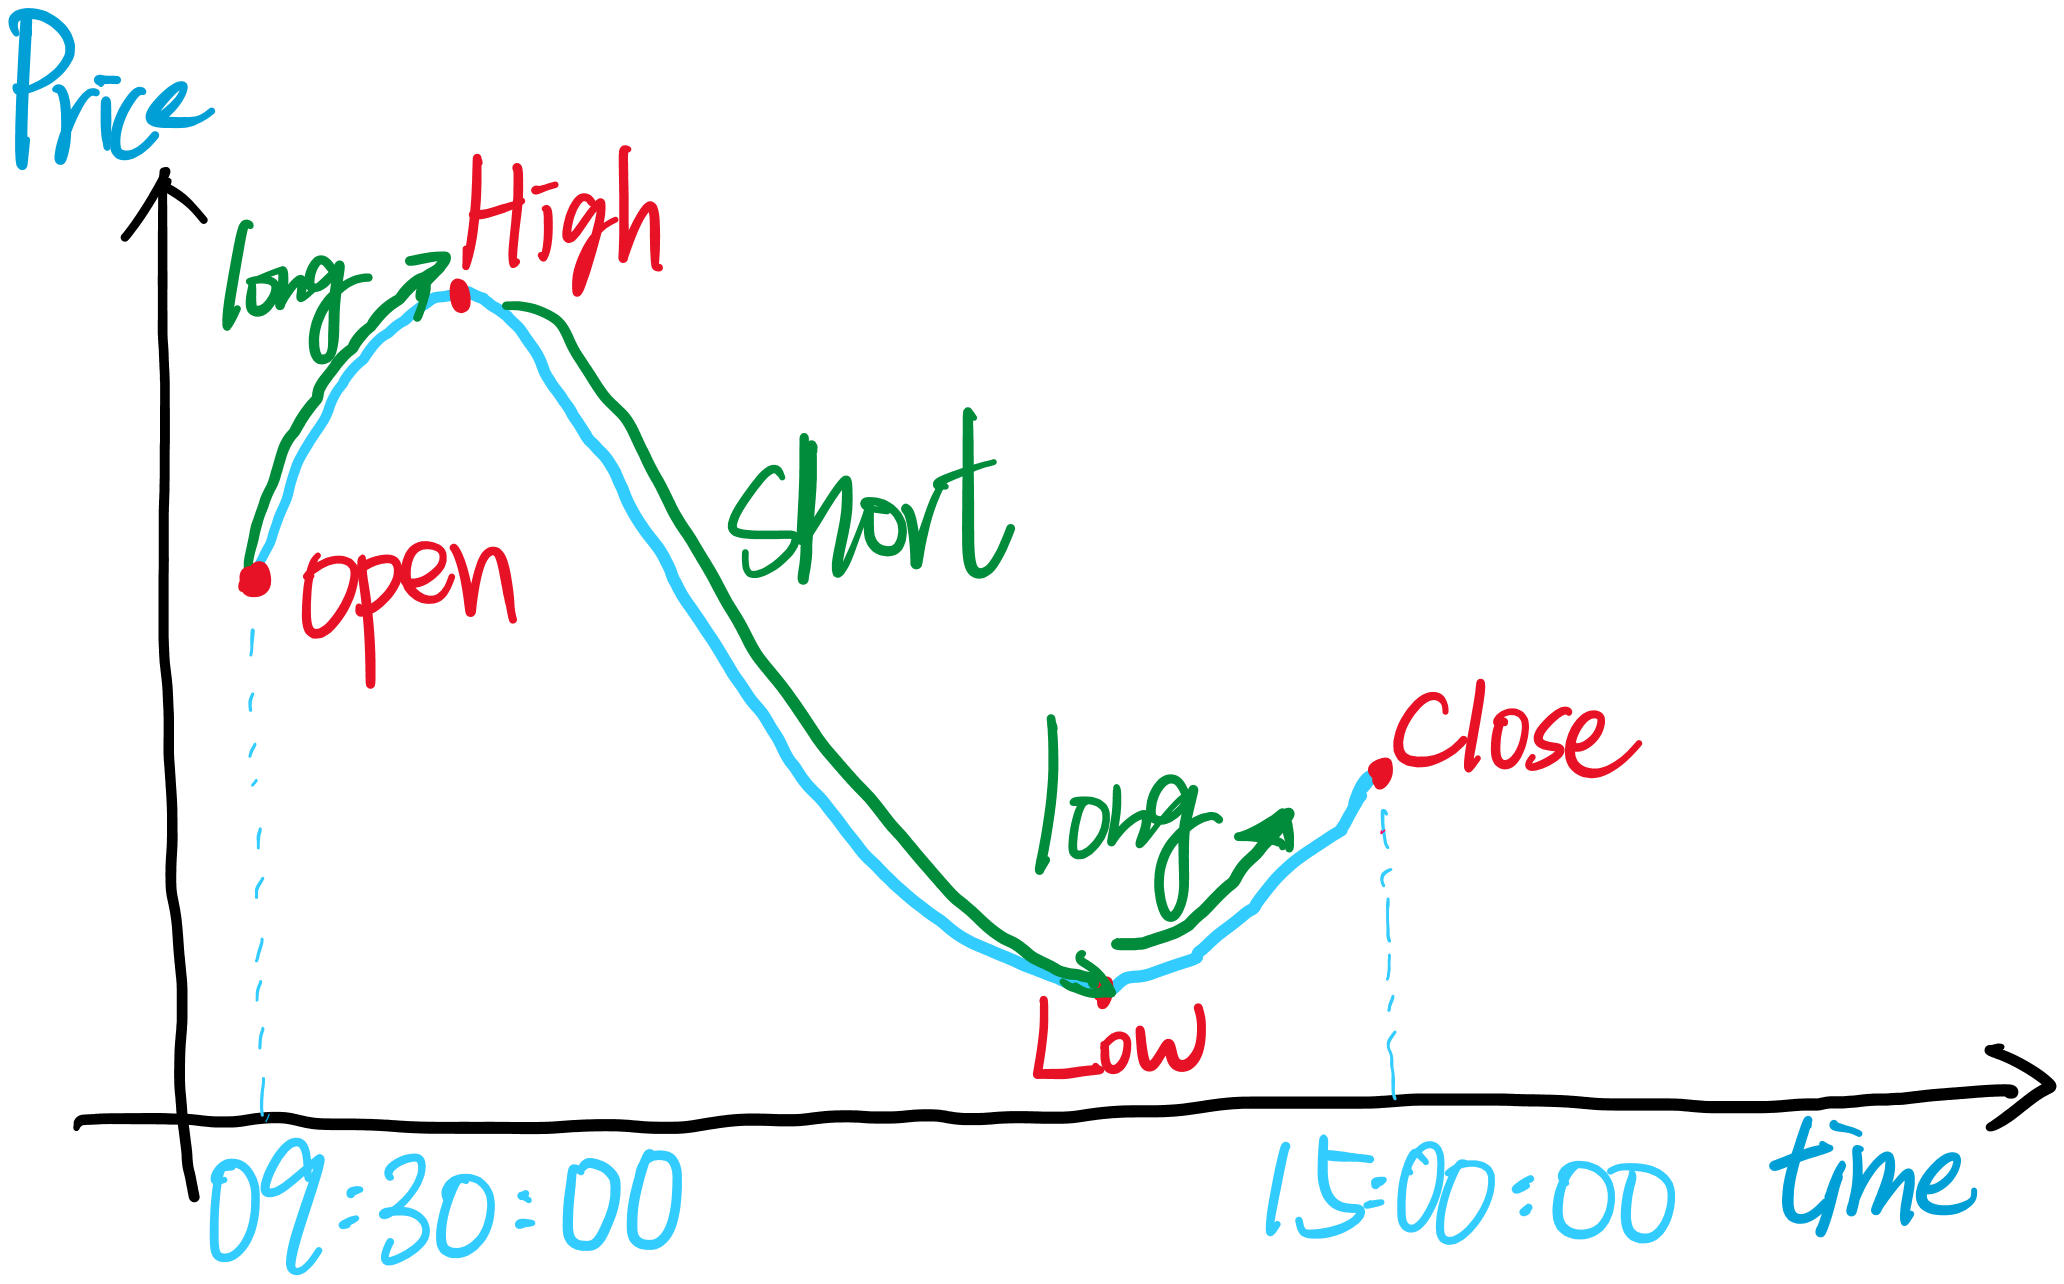
\includegraphics[width=8cm]
    {BC_demo3}
    \caption{  intra-day greedy actions as expert actions }
    \label{fig:  Using intra-day greedy actions as expert actions }
\end{figure}

The next is about the loss function. You could see the down figure.
Since Behavior cloning is a kind of supervised learning approach, we take the square of the policy difference between actor and expert. \\
In addition, we apply the Q-filter technique.
That is, we record BC Losses only when the critic Q indicates that the expert actions perform better than the actor action.\\
Finally, as shown by the picture below, we combine the BC loss with the original objective function, and calculate its policy gradient for updating the actor.


\begin{figure}[h!]
    \center
    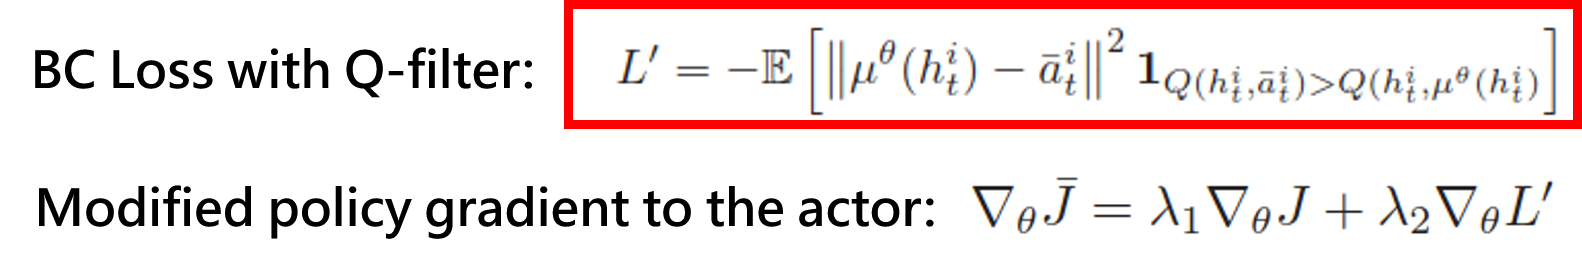
\includegraphics[width=9cm]
    {BC}
    % \caption{ Q-filter and modified policy gradient }
    \label{fig: The IF IC}
\end{figure}





\newpage
\section{Detailed Implementation}
\label{section:implementation}
Please explain your implementation in detail. You may do this with the help of pseudo code or a figure of system architecture. Please also highlight which parts of the algorithm lead to the most difficulty in your implementation.


\subsection{Whole iRDPG Algorithm}
iRDPG proposed by \cite{liu2020adaptive} is abbreviation of imitative Recurrent Deterministic Policy Gradient. As the name suggests, which improve RDPG by introducing imitation learning. 

As the figure showed bellow. We can see the architecture of iRDPG. The bottom part is the market observation.  It will first be fed into the GRU layer to encode its historical information, and then the GRU hidden state will be send into the Agent. In the agent module, the behavior cloning loss is used to supervised the actor. And the Demonstration Buffer allows Actors to learn the experience of expert.

\begin{figure}[h!]
    \center
    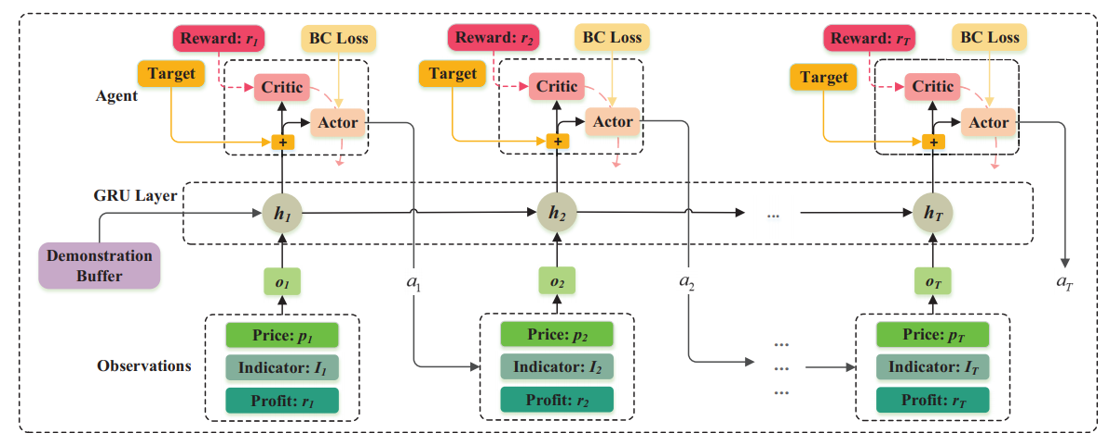
\includegraphics[width=14cm]
    {irdpg}
    \caption{The overview of iRDPG model}
    \label{fig: The iRDPG model}
\end{figure}



\subsection{Experiment Setup}
In our experiment, we use minute-bar OHLC prices data of futures, 
i.e. minute-frequent futures data(IF and IC) \cite{joinQuant}. \\
Training set starts from 2016/01/01 to 2018/05/08. \\
Testing set spans from 2018/05/09 to 2019/05/08. \\
Transaction fee  : 2.3*10-5 \\
The constant slippage: 0.2 \\
Initialize account: 500000 CNY\\
Each training episode will be broken off once positions are lost around 30\% or lacking margin.

\begin{figure}[h!]
    \center
    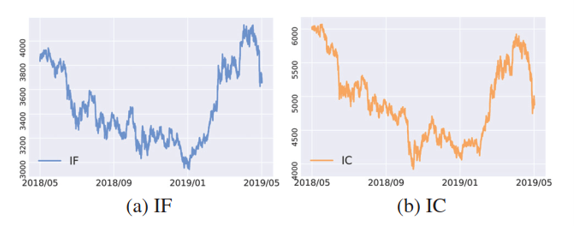
\includegraphics[width=10cm]
    {IFIC_2}
    \caption{ IF and IC stock-index futures in our test set}
    \label{fig: The IF IC}
\end{figure}

* The IF data are based on the index calculated on account of the prices of the top 300 stocks from both 
Shanghai and Shenzhen exchange centers. \\
* The IC data are based on another similar index, which focuses on the stocks with mid and small capitalization. \\


\subsection{Dual Thrust Strategy}

It is famous and has been commonly used in futures, forex, and equity markets.
As the introduction in the Demonstration Buffer, we select the Dual Thrust strategy as the demonstration trading policy. First, the DT determines a reasonable price oscillation Range, and the Range is calculated in this way by using OHLC in the previous n periods.
Then use this range to determine the buyline and sellline. Finally, if the price goes beyond the buyline, a long position will be taken.
And the short position will be taken if the price goes under the sellLine.

The long signal is calculated by Buyline (cap)=open+K1×Range. \\
The short signal is calculated by SellLine (floor) = open–K2×Range \\
, where K1 and K2 are the parameters. When K1 is greater than K2, it is much easier to trigger the long signal and vice versa. 
The idea of Dual Thrust is similar to a typical breakout system, However, dual thrust uses the historical price to construct update the look back period - theoretically making it more stable in any given period.


\begin{figure}[h!]
    \center
    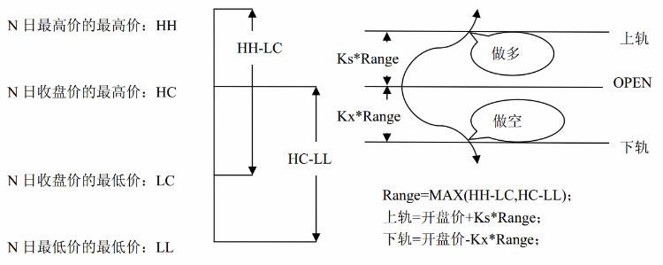
\includegraphics[width=12cm]
    {DT_1}
    \caption{Dual Thrust Strategy}
    \label{fig: The DT1}
\end{figure}

% \begin{figure}[h!]
%     \center
%     \includegraphics[width=10cm]
%     {DT_2}
%     % \caption{Dual Thrust Strategy}
%     \label{fig: The DT2}
% \end{figure}

\subsection{The Most Difficulties in Our Implementation}
First, no member is familiar with the market characteristics and trading rules of China stock index futures, but fortunately the minute-frequent price data can be friendly downloaded on JoinQuant website for a student registration member. 
Beside, although the POMDP framework can better represent the noisy minute-frequent financial data, it is still quite a challenge to tune the agent. \\
No source code, the simulated trading environment is also coded from scratch, its complexity is beyond our imagination. Besides, although the differential sharp ratio (DSR) looks having nice property for considering both dynamically changing return and risk, but the formula often faces zero values for both numerator and denominator and how to set the proper value of adaptation rate $\eta$.\\
The ablation experiment takes so much time because the hyperparameters are quite different for each setting. For example, when adding the new imitation techniques to the original RDPG, the characteristics for each training process are very different, the trial and error need much efforts. \\







\newpage
\section{Empirical Evaluation}
\label{section:evaluation}
Please showcase your empirical results in this section. Please clearly specify which sets of experiments of the original paper are considered in your report. Please also report the corresponding hyperparameters of each experiment.

\subsection{Training History}

\begin{figure}[h!]
    \center
    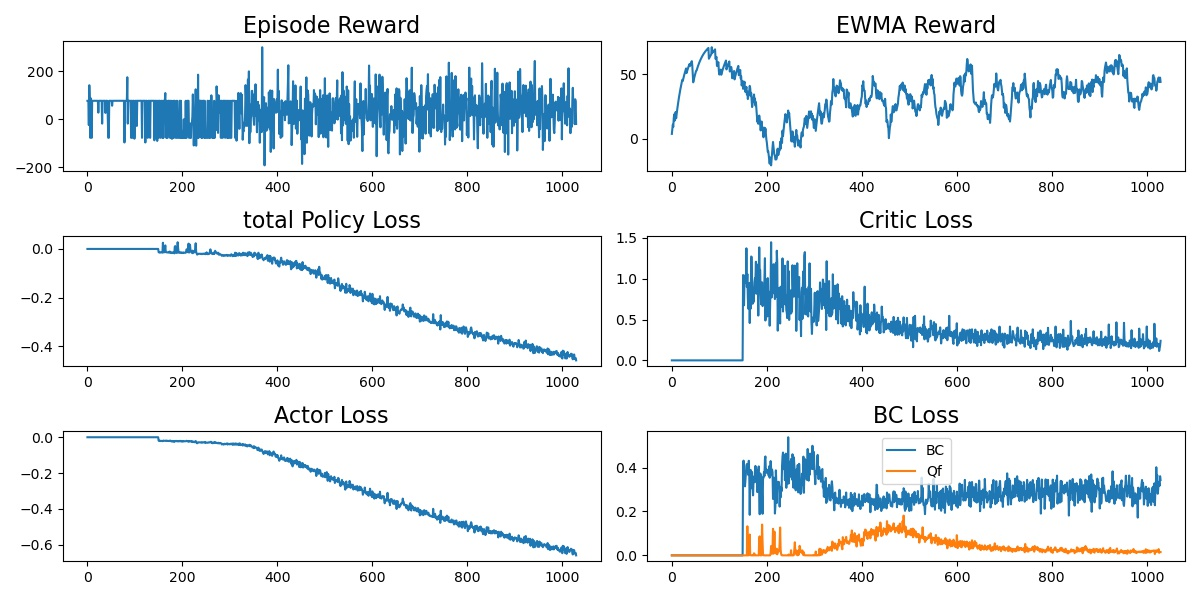
\includegraphics[width=15cm]
    {TrainCurve}
    \caption{The training curve}
    \label{fig: The training curve}
\end{figure}

This paper didn’t show any training history, so here shows our training results for the iRDPG agent. The total policy loss is the summation of actor loss and BC loss after Q-filter. For the first 150 episodes, we only conduct sampling without training.  So in the early training stage, the EWMA reward is relatively high because these are expert demonstrations. Then, from the BC Loss figure, the yellow curve is the BC loss after Q-filter. And we can see that the yellow curve decreases much, even though the original BC loss doesn’t decrease. It is evident that the iRDPG agent learns better policies than the expert as the training time goes by.


\subsection{Hyperparameters}

\begin{figure}[h!]
    \center
    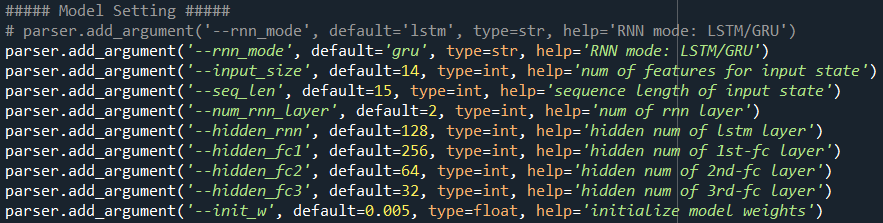
\includegraphics[width=15cm]
    {param_model}
    \caption{Parameters for agent model}
    \label{fig: param_model}
\end{figure}

Figure 6 presents the agent model setting. we can ether set the RNN layer as LSTM or GRU with two layers. The input size means input features which contain OHLC prices, buyline-selline of Dual Thrust, simple moving averages with previous 7 and 56 minites, RSI, KD, MACD, account profit and margin, etc. And the state sequence length is 15 minutes. In addition, both actor and critic has same three hidden layers but different input and output.

\begin{figure}[h!]
    \center
    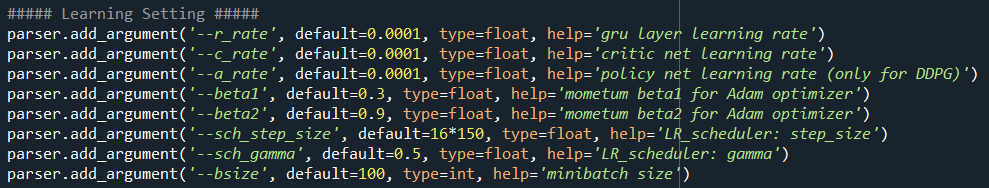
\includegraphics[width=15cm]
    {param_learning}
    \caption{Parameters for Adam optimizer and LR-scheduler}
    \label{fig: param_learning}
\end{figure}


\begin{figure}[h!]
    \center
    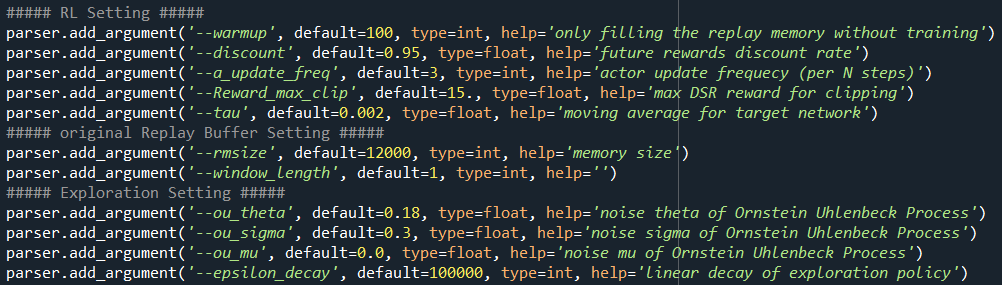
\includegraphics[width=15cm]
    {param_RL}
    \caption{Parameters for RL-algorithm, and random-process}
    \label{fig: param_RL}
\end{figure}

In figure 8, we set the warmup to be 100 episodes. Discount rate is 0.95. The soft replace rate is 0.002. Note, we update the actor every three step after updating the critic. Besides, the exploration is based on the Ornstein Uhlenbeck Process. 

\begin{figure}[h!]
    \center
    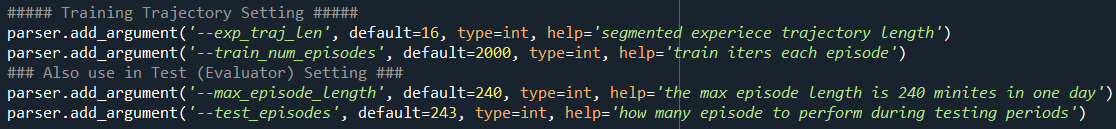
\includegraphics[width=15cm]
    {param_traj}
    \caption{Parameters for training trajectory}
    \label{fig: param_traj}
\end{figure}

In figure 9, the maximum steps of each episode is 240 since there are 240 trading minutes each day. And we segment every 16 steps to form an experience for train the recurrent DPG network. In addition, there are 243 trading days in the testing period.

\begin{figure}[h!]
    \center
    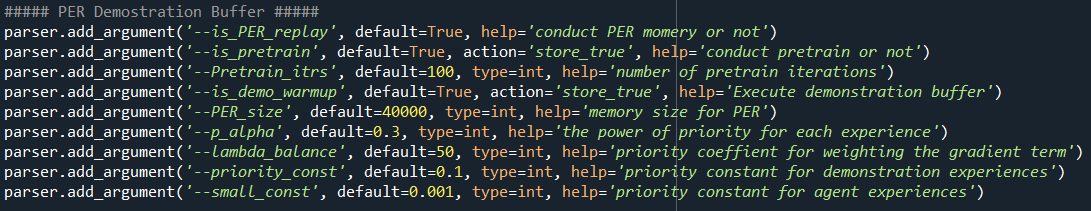
\includegraphics[width=15cm]
    {param_PER}
    \caption{Parameters for demonstration buffer and PER}
    \label{fig: param_PER}
\end{figure}

\begin{figure}[h!]
    \center
    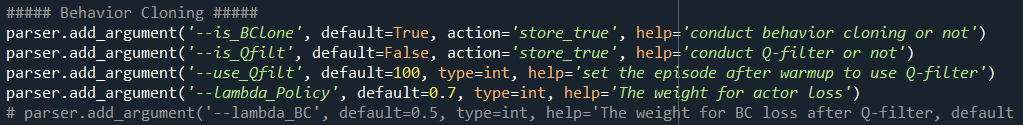
\includegraphics[width=15cm]
    {param_BC}
    \caption{Parameters for behavior cloning}
    \label{fig: param_BC}
\end{figure}


\begin{figure}[h!]
    \center
    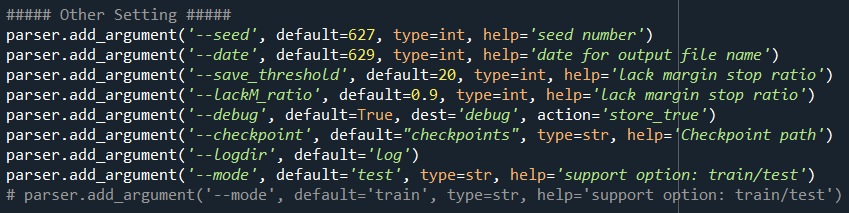
\includegraphics[width=15cm]
    {param_other}
    \caption{Parameters for other settings}
    \label{fig: param_other}
\end{figure}


\subsection{Ablation Experiments}

\begin{figure}[h!]
    \center
    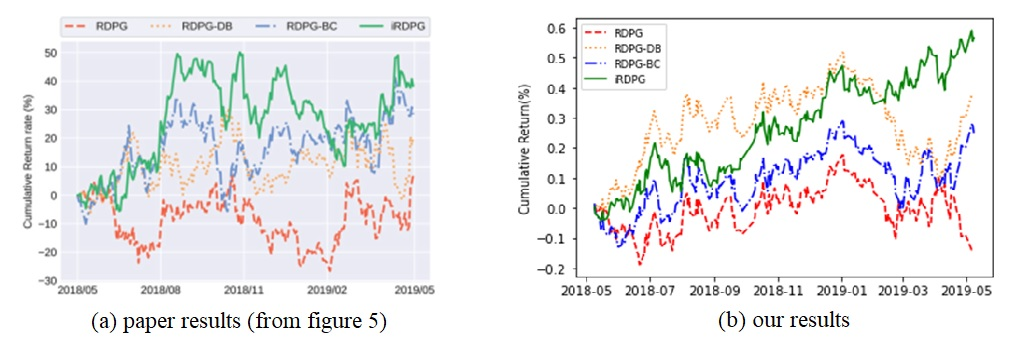
\includegraphics[width=15cm]
    {ablation}
    \caption{Cumulative return rates of ablation methods}
    \label{fig: ablation}
\end{figure}


This figure shows the comparison of ablation experiments. The LHS are the paper results (from Figure 5), and the RHS are our results. Both figures are the trading simulations by applying the trained agent to the one year test data (IF stock index futures from 2018/5/9 to 2019/5/8). And the four settings are RDPG, RDPG plus demonstration buffer (RDPG-DB), RDPG plus behavior cloning (BC), and the comprehensive iRDPG. Obviously, we can see that both results have similar trend, that is the iRDPG got the best trading performance. Also, we can find that if we train the RDPG without imitation technique, the RDPG trading performances are both not stable as shown by these two red curve.


\begin{figure}[h!]
    \center
    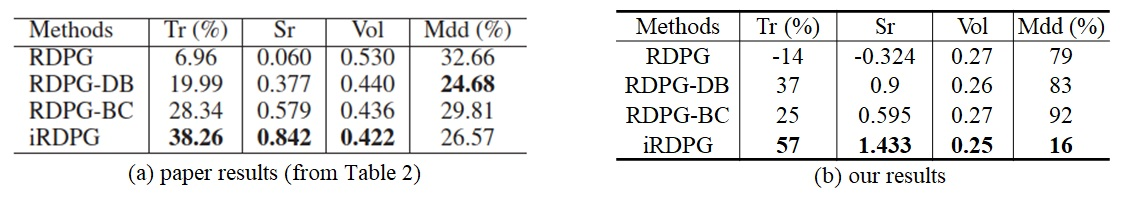
\includegraphics[width=13cm]
    {ablationTable}
    \caption{Ablation experiments of IF}
    \label{fig: ablationTable}
\end{figure}

The above two tables are the comparison of ablation trading performances on the following most widely used criteria. The LHS are the paper results (from Table 2), and the RHS are our results. Both tables are the trading performances by applying the trained agent to the one year test data (IF stock index futures from 2018/5/9 to 2019/5/8). Again, we can find that the iRDPG got the best performance. 

\begin{itemize}
    \item  Total return rate $\textbf{Tr}:=\frac{P_{end}-P_{start}}{P_{start}}$ ($P$ is the total value of the position and cash).
    \item Sharpe ratio $\textbf{Sr}:=\frac{\EX(\textbf{r})}{\sigma[\textbf{r}]}$ considers benefits and risks synthetically and reflects the excess return over unit systematic risk.
    \item  Volatility $\textbf{Vol}:=\sigma[\textbf{r}]$ (r denotes the historical sequence of return rate.) measures the uncertainty of return rate and reflects the risk level of strategies.
    \item  Maxium Drawdown $\textbf{Mdd}:=max\frac{(P_{i}-P_{j})}{(P_{i})},j>i$ measures the largest decline in history and shows the worst possible scenario.
\end{itemize}


\subsection{Generalization Ability}

\begin{figure}[h!]
    \center
    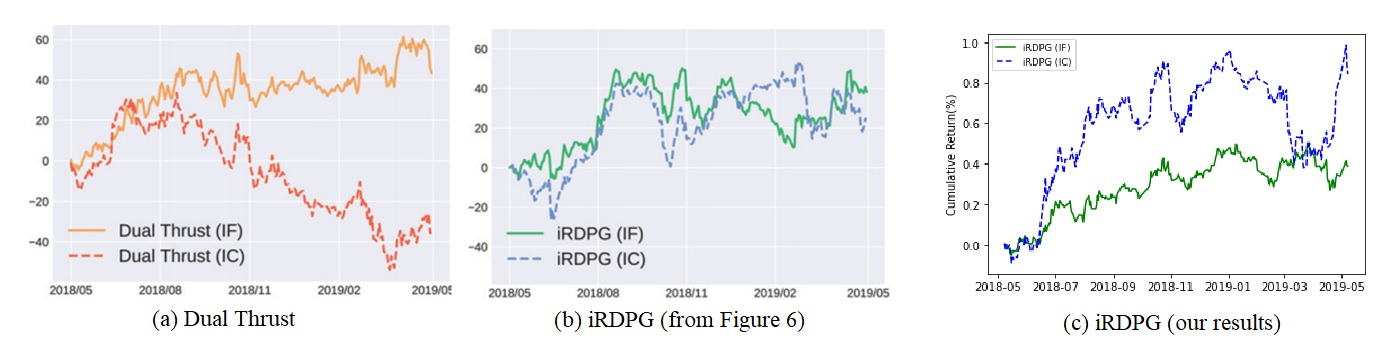
\includegraphics[width=15cm]
    {generalizability}
    \caption{Generalizability of iRDPG on IF and IC}
    \label{fig: generalizability}
\end{figure}

These figures present the generalizability of iRDPG agent. Figure(15-a) shows that if we apply the best parameter of Dual Thrust Strategy from IF to IC, it will fail as shown by the red curve. However, such failure will not happen by using the iRDPG agent. The iRDPG agent is trained in the IF training set and is tested in the IF and IC test set respectively. Figure(15-b) is the results from the paper Figure6, and Figure (15-c) is our implementation results. It is obvious that the agent got nice trading performance on both IF data and IC data. And such a trend in our results is consistent with the paper results. (Note: The reason why we can not successfully derive these results before the oral presentation on 6/23 is that we had different normalization settings for agent state value on IF and IC.)


\section{Conclusion}
\label{section:conclusion}
Please provide succinct concluding remarks for your report. You may discuss the following aspects:
\begin{itemize}
    \item The potential future research directions
    \item Any technical limitations
    \item Any latest results on the problem of interest
\end{itemize}

\subsection{Consistent Conclusions with the Original Paper}
1. Imitation learning techniques is successfully introduced to balance the exploration and exploitation of the trading agent.\\
2. The iRDPG suggests that the trading agent can benefit from experiences of classical trading strategies such as Dual Thrust Strategy.\\
3. The profitability and ability to resist risks of iRDPG were verified.\\
4. Comparison experiments provided its generalizability for different financial markets.\\


\subsection{Technical Limitation and Possible Future works}
Although the iRDPG agent can finally learn better policies than expert, this framework still needs well performed demonstrations in the early training stage. Therefore, in the future, maybe it can try other technique such as "policy optimization from demonstration (POfD)" (\cite{kang2018policy}), which allows imperfect expert policies in the beginning.



{
\small
\bibliographystyle{unsrtnat}
\bibliography{reference}
}


\end{document}

